
\documentclass[12pt,letterpaper]{article}

\usepackage[margin=1in]{geometry}
\usepackage{amsmath,amssymb}
\usepackage{booktabs}
\usepackage{graphicx}
\usepackage{hyperref}
\usepackage{enumitem}
\usepackage{caption}
\usepackage{array}
\usepackage{parskip}
\usepackage{float}
\usepackage{longtable}

\hypersetup{
    colorlinks=true,
    linkcolor=blue,
    urlcolor=blue
}

\begin{document}

\begin{titlepage}
\centering
\vspace*{1.2cm}

{\Large MIE312: Lab 3\par}
\vspace{0.5em}
{\Huge\bfseries External Flow: Lift and Drag on Airfoils\par}
\vspace{1.2em}

{\Large Department of Mechanical and Industrial Engineering\par}
{\Large University of Toronto\par}
\textcolor{white}{\Large Prepared by: Prof. Sullivan} \\
{\Large Fall 2026}

\vfill

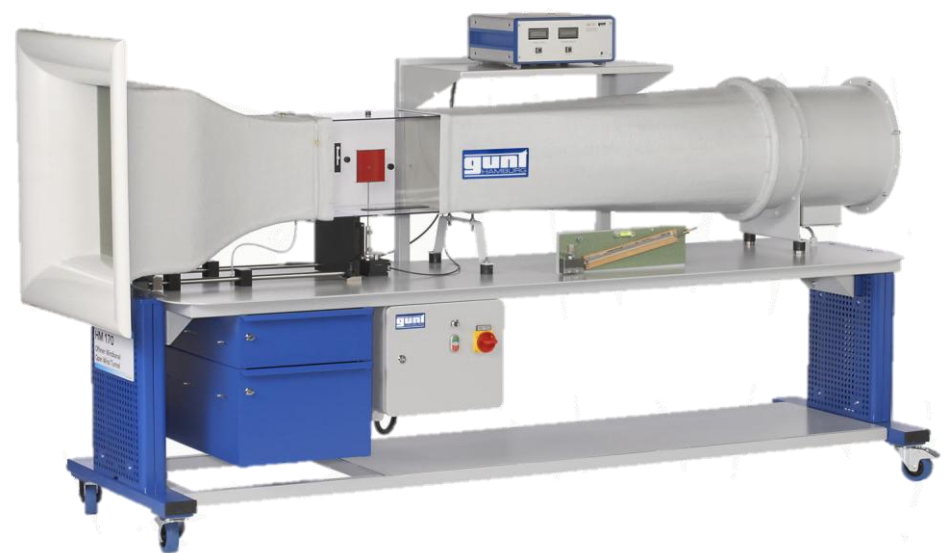
\includegraphics[width=0.78\textwidth]{Lab3_Figures/Lab3_cover.png}

\vfill

\begin{tabular}{|p{0.32\textwidth}|p{0.38\textwidth}|}
\hline
Teaching Assistant: & Arash Zargar \\ \hline
Email: & \texttt{a.zargar@mail.utoronto.ca} \\ \hline
\end{tabular}

\vfill
\end{titlepage}

\section*{Companion Notebook}

A Google Colab notebook accompanies this lab manual. It automates coefficient calculations, generates report-ready lift and drag plots, identifies the stall region, and compares the airfoil data with simplified drag models once the measured data are entered.

\begin{center}
\href{https://colab.research.google.com/github/pierresullivan/mie312-labs/blob/main/lab3-aero/MIE312_Lab3_External_Flow.ipynb}{\textbf{Open the MIE312 Lab 3 Colab Notebook}}
\end{center}

\subsection*{How students should use the notebook}
\begin{enumerate}[leftmargin=*, label=\arabic*.]
    \item Open the notebook and save a personal copy.
    \item Run the setup cells first so the constants, geometry, and helper functions are defined.
    \item Enter the measured angle, raw $F_y$ lift-channel reading, drag-channel reading, and fan velocity values in the data-entry table.
    \item Run the remaining cells to compute corrected drag, Reynolds number, \(C_L\), and \(C_D\), and to generate the report-quality plots.
    \item Copy the generated tables, plots, and discussion prompts into the final report as needed.
\end{enumerate}

\vspace{1em}

\hrule
\vspace{1em}

\section{Objective}
The objectives of this lab experiment are to:
\begin{itemize}[leftmargin=*]
    \item determine the lift and drag curves for the given airfoil,
    \item estimate the stall onset region of the given airfoil,
    \item compare drag force with that expected from a simple flat-plate and bluff-body models under the same flow conditions,
    \item identify key design elements in the use of airfoils,
    \item explore practical applications of airfoils in modern engineering practice.
\end{itemize}

\section{Experimental Setup}
Figure~\ref{fig:windtunnel} shows the wind tunnel used in this experiment. The original lab manual identifies the following major components:
\begin{enumerate}[leftmargin=*, label=\arabic*.]
    \item Inlet contour
    \item Flow straightener
    \item Nozzle
    \item Measuring section
    \item Drag body (airfoil)
    \item Force sensor and angular adjuster
    \item Display and control unit
    \item Diffuser
    \item Switch cabinet
    \item Inclined tube manometer
    \item Axial fan
\end{enumerate}

\begin{figure}[H]
    \centering
    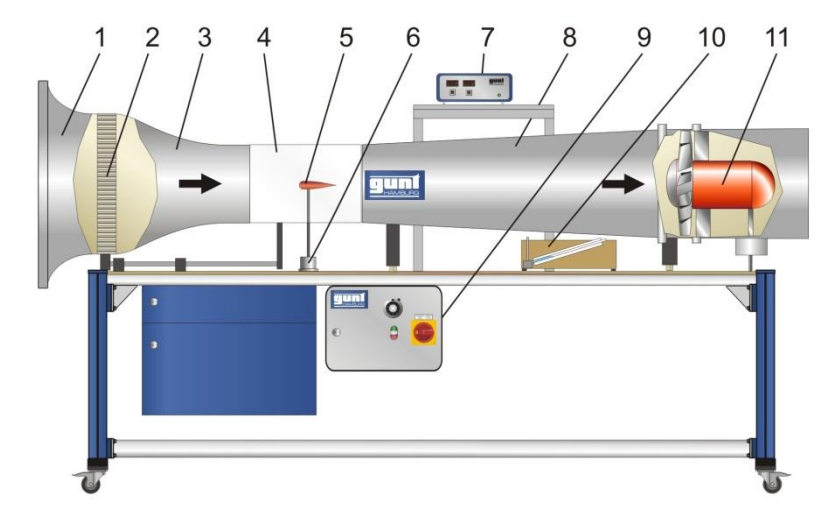
\includegraphics[width=0.92\textwidth]{Lab3_Figures/Lab3_schematic.png}
    \caption{Wind tunnel schematic showing the major components of the external-flow apparatus.}
    \label{fig:windtunnel}
\end{figure}

\subsection*{Student interpretation of the apparatus}
The apparatus is designed to generate a controlled external airflow over a model airfoil in the measuring section. The nozzle accelerates the air, the measuring section allows the airfoil to be observed and rotated, and the force sensor resolves the aerodynamic force into two components. These measured components are then used to infer lift and drag as functions of angle of attack.

The inclined tube manometer provides the test-section velocity, while the airfoil orientation is controlled by the angular adjustment mechanism. Because the airfoil is mounted using a holder, the measured drag includes both the airfoil drag and the holder contribution; this is why a holder correction is required in the analysis.

\subsection*{Important dimensions}
The original lab manual provides the following dimensions:
\begin{itemize}[leftmargin=*]
    \item \textbf{Measurement section:}
    \begin{itemize}
        \item Length: \(420~\text{mm}\)
        \item Cross-sectional area: \(292 \times 292~\text{mm}\)
    \end{itemize}
    \item \textbf{Airfoil:}
    \begin{itemize}
        \item Chord length: \(c = 0.10~\text{m}\)
        \item Thickness: \(t = 15~\text{mm} = 0.015~\text{m}\)
        \item Planform area: \(A = 0.01~\text{m}^2\) \((0.10~\text{m} \times 0.10~\text{m})\)
    \end{itemize}
    \item \textbf{Holder:}
    \begin{itemize}
        \item Length: \(0.31~\text{m}\)
        \item Diameter: \(4~\text{mm}\)
        \item Front-area drag parameter: \(C_DA_{\text{front}} = 0.000125~\text{m}^2\)
    \end{itemize}
\end{itemize}

\begin{figure}[H]
    \centering
    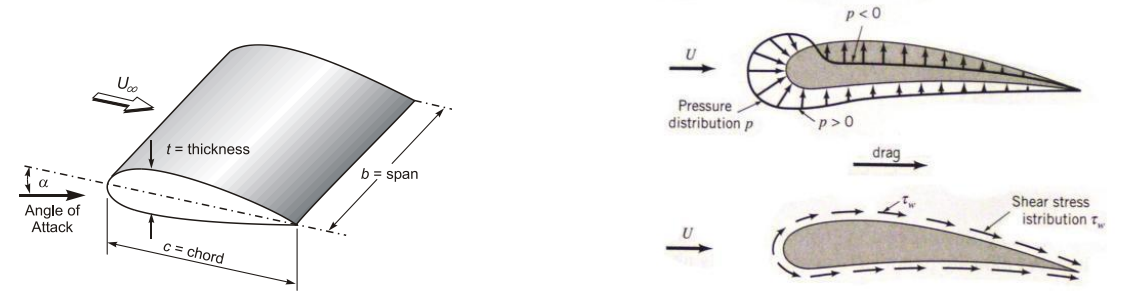
\includegraphics[width=0.72\textwidth]{Lab3_Figures/Lab3_airfoil.png}
    \caption{Airfoil geometry and notation used in the experiment.}
    \label{fig:airfoil-geometry}
\end{figure}

\section{Theoretical Background}

\subsection{Lift and Drag Forces}
When a body is placed in an external flow, the fluid exerts distributed pressure and shear stresses on its surface. These surface forces can be resolved into two resultant components:
\begin{itemize}[leftmargin=*]
    \item \textbf{Drag force, \(F_D\):} the component parallel to the upstream flow direction,
    \item \textbf{Lift force, \(F_L\):} the component perpendicular to the upstream flow direction.
\end{itemize}

For an airfoil, both pressure distribution and viscous shear contribute to the net aerodynamic force. In many practical external-flow problems, pressure effects dominate lift, while both pressure and viscous effects contribute to drag.

\begin{figure}[H]
    \centering
    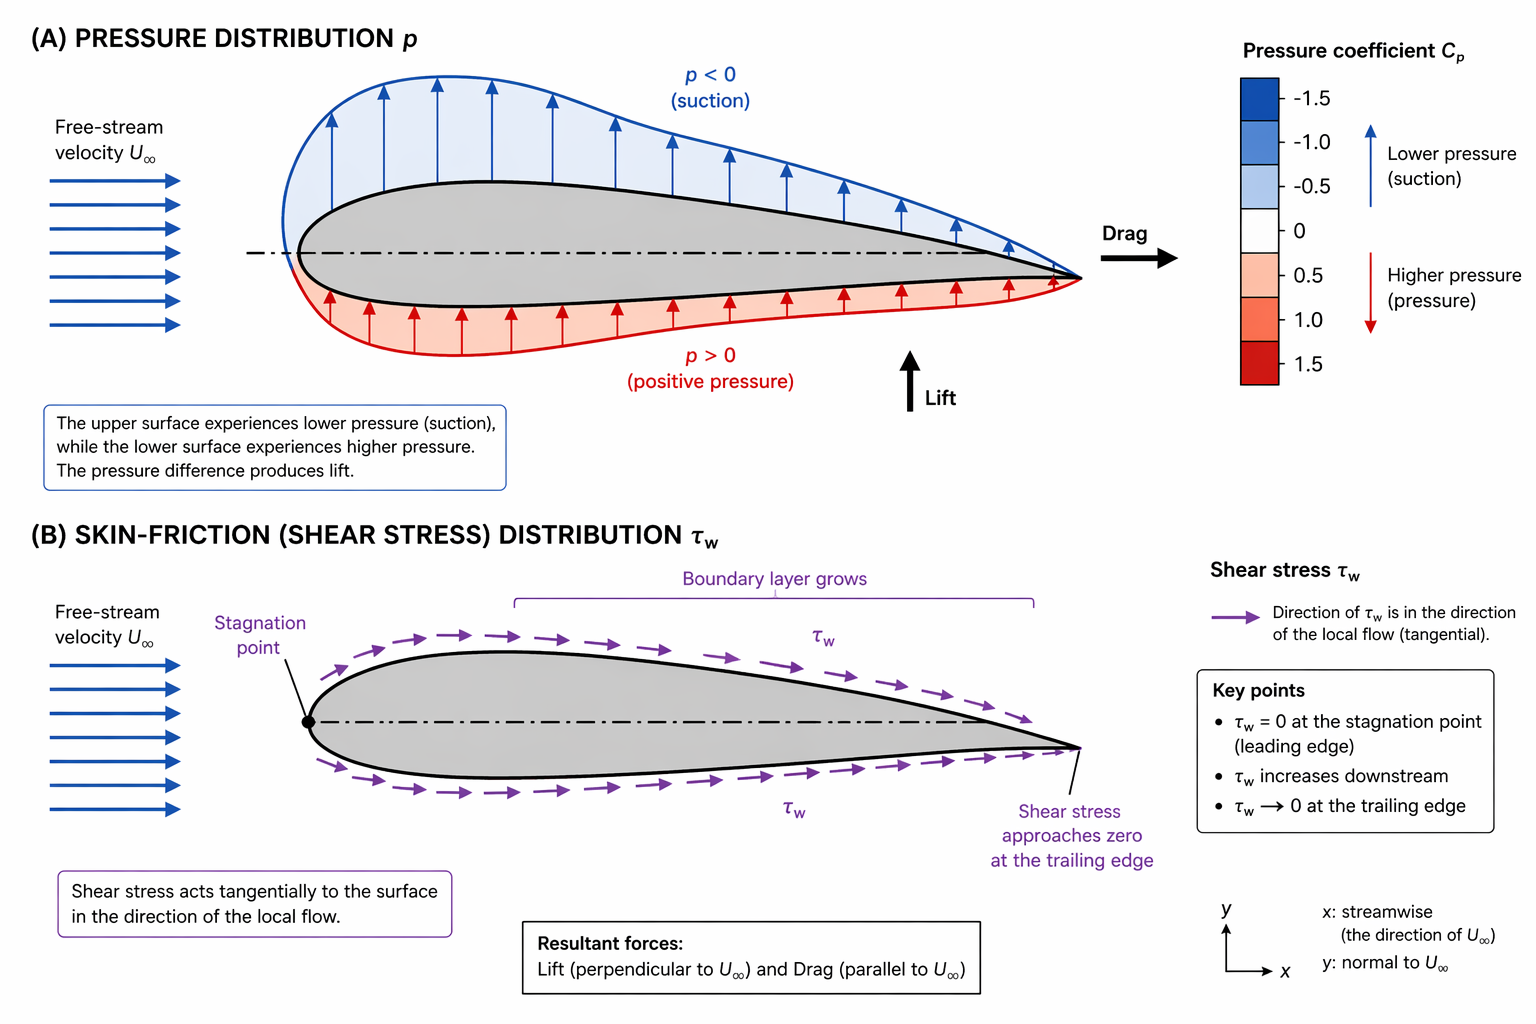
\includegraphics[width=0.92\textwidth]{Lab3_Figures/pressure_shear.png}
    \caption{Pressure and shear-stress contributions to lift and drag on an airfoil.}
    \label{fig:pressure-shear}
\end{figure}

\subsection{Dynamic Pressure and Aerodynamic Coefficients}
Because the force depends strongly on velocity, density, and size, it is standard practice to define dimensionless coefficients using the dynamic pressure:
\begin{equation}
q = \frac{1}{2}\rho V^2
\label{eq:dynamicpressure}
\end{equation}
where:
\begin{itemize}[leftmargin=*]
    \item \(\rho\) is the air density,
    \item \(V\) is the upstream air velocity in the test section.
\end{itemize}

The lift and drag coefficients are then defined as
\begin{equation}
C_L = \frac{F_L}{\frac{1}{2}\rho V^2 A},
\qquad
C_D = \frac{F_D}{\frac{1}{2}\rho V^2 A}
\label{eq:clcd}
\end{equation}
where \(A\) is the chosen reference area. In this lab, the given planform area of the airfoil is
\[
A = c\,b = 0.10 \times 0.10 = 0.01~\text{m}^2.
\]

\subsection{Angle of Attack}
The angle of attack, denoted \(\alpha\), is the angle between the incoming flow direction and the airfoil chord line. It is one of the most important parameters in airfoil performance:
\begin{itemize}[leftmargin=*]
    \item As \(\alpha\) increases from small values, lift generally increases.
    \item Drag also increases with \(\alpha\), although often more gradually at first.
    \item Beyond a critical angle, the flow begins to separate significantly from the suction side of the airfoil, causing \emph{stall}.
\end{itemize}

\subsection{Qualitative Airfoil Behaviour}
At low to moderate angles of attack:
\begin{itemize}[leftmargin=*]
    \item the pressure on the lower surface is relatively high,
    \item the pressure on the upper surface is relatively low,
    \item the resulting pressure difference creates upward lift.
\end{itemize}

As the angle of attack increases further, the adverse pressure gradient on the upper surface becomes stronger. Eventually the boundary layer can no longer remain attached, and flow separation develops over the suction side of the airfoil. This leads to:
\begin{itemize}[leftmargin=*]
    \item a sharp decrease or plateau in lift,
    \item a rapid increase in drag,
    \item unsteady behaviour and visible vibration or separation in the test section.
\end{itemize}

This condition is called \textbf{stall}, and the associated angle is called the \textbf{stall angle}.

\subsection{Why the Lift Curve and Drag Curve Matter}
The lift curve \(F_L(\alpha)\) or \(C_L(\alpha)\) describes how effectively the airfoil generates useful normal force as the angle changes. The drag curve \(F_D(\alpha)\) or \(C_D(\alpha)\) describes the aerodynamic penalty required to generate that lift.

For design purposes:
\begin{itemize}[leftmargin=*]
    \item high lift is desirable when large normal force is required,
    \item low drag is desirable for aerodynamic efficiency,
    \item the best operating angle is often not the angle of maximum lift, but rather the angle that gives the most desirable balance between lift and drag.
\end{itemize}

\subsection{Lift-to-Drag Ratio}
A common measure of aerodynamic efficiency is the lift-to-drag ratio:
\begin{equation}
\frac{L}{D} = \frac{F_L}{F_D} = \frac{C_L}{C_D}
\label{eq:ldratio}
\end{equation}
A larger value of \(L/D\) usually indicates a more aerodynamically efficient operating condition. Students should be careful, however: the angle of maximum \(L/D\) is not necessarily the same as the angle of maximum lift.

\subsection{Velocity Measurement and Reynolds Number}
The test velocity is set to approximately \(15~\text{m/s}\) using the inclined tube manometer. Once the velocity is known, the Reynolds number for the airfoil is
\begin{equation}
Re = \frac{\rho V c}{\mu}
\label{eq:reynolds}
\end{equation}
where:
\begin{itemize}[leftmargin=*]
    \item \(c = 0.10~\text{m}\) is the chord length,
    \item \(\mu\) is the dynamic viscosity of air.
\end{itemize}

Students may also use the equivalent form
\begin{equation}
Re = \frac{Vc}{\nu}
\label{eq:reynolds-kin}
\end{equation}
if the kinematic viscosity \(\nu\) is used instead.

For consistency between the manual and the companion notebook, use dry-air properties at \(20^\circ\mathrm{C}\) and \(1~\mathrm{atm}\):
\[
\rho = 1.204~\mathrm{kg/m^3},
\qquad
\mu = 1.81\times10^{-5}~\mathrm{Pa\,s}.
\]
These values are treated as constant over the experiment. The measured velocity at each angle of attack should be used in the Reynolds-number and aerodynamic-coefficient calculations.

The Reynolds number is important because it affects:
\begin{itemize}[leftmargin=*]
    \item boundary-layer development,
    \item flow separation,
    \item drag behaviour,
    \item stall characteristics.
\end{itemize}

\subsection{Holder Drag Correction}
The drag measured by the sensor is not due solely to the airfoil. The holder also contributes drag. Therefore:
\begin{equation}
F_{D,\text{net}} = F_{D,\text{measured}} - F_{D,\text{holder}}
\label{eq:dragcorrection}
\end{equation}
The holder drag can be estimated from the given front-area drag parameter:
\begin{equation}
F_{D,\text{holder}} = \frac{1}{2}\rho V^2\left(C_DA\right)_{\text{front}}
\label{eq:holderdrag}
\end{equation}
with
\[
\left(C_DA\right)_{\text{front}} = 0.000125~\text{m}^2.
\]

This correction must be shown clearly in the report, since the corrected drag is the quantity used to calculate the drag coefficient of the airfoil itself.


\subsection{Lift-Force Sign Convention}
With the axis configuration used in the GUNT software for this lab, upward aerodynamic lift is displayed as a \emph{negative} value of the raw \(F_y\) channel. For the analysis and for the companion notebook, define positive physical lift as
\begin{equation}
F_L = -F_y.
\label{eq:lift-sign}
\end{equation}
Thus a raw reading such as \(F_y=-0.80~\text{N}\) corresponds to \(F_L=+0.80~\text{N}\). Preserve the raw reading in your data table, but convert to the physical sign convention before calculating \(C_L\), \(L/D\), the stall point, or the angle of maximum lift. If the software axis direction has been reconfigured during your session, verify the sign experimentally and document the convention used.

\subsection{Comparison with Simple Bodies}
In the analysis section, students compare airfoil drag to flat-plate or bluff-body estimates. The purpose is not to claim that the airfoil \emph{is} a simple flat-plate and bluff-body models, but to develop physical intuition:
\begin{itemize}[leftmargin=*]
    \item At \(0^\circ\), the airfoil behaves more like a streamlined body with relatively small frontal thickness.
    \item At \(90^\circ\), the airfoil behaves much more like a bluff body with large projected area. For the simplified comparison used in this lab, model the airfoil as a thin two-dimensional plate normal to the flow, use the projected area \(A_{90}=0.10\times0.10=0.010~\mathrm{m^2}\), and adopt \(C_D=1.9\). This is a prescribed idealized comparison coefficient, representative of a normal flat plate, rather than an airfoil-specific measured value; see Hoerner (1965).
\end{itemize}

These comparisons help explain why orientation matters so strongly in external-flow drag problems. For both the \(0^\circ\) and \(90^\circ\) comparisons, use the velocity measured at the corresponding angle rather than a single common reference velocity.

\subsection{What students should calculate from the raw data}
For each angle of attack, students should determine:
\begin{enumerate}[leftmargin=*, label=\arabic*.]
    \item raw lift-sensor reading \(F_y\) and converted physical lift \(F_L=-F_y\),
    \item measured drag force \(F_{D,\text{measured}}\),
    \item holder drag \(F_{D,\text{holder}}\),
    \item corrected or net airfoil drag \(F_{D,\text{net}}\),
    \item lift coefficient \(C_L\),
    \item drag coefficient \(C_D\),
    \item optionally the lift-to-drag ratio \(L/D\).
\end{enumerate}

\section{Procedure}

\subsection*{Safety}
\textbf{CAUTION:} Do not stand in front of or behind the wind tunnel while it is in use. Before beginning the experiment, ensure that both areas are clear.

\textbf{Note:} When pressing buttons on the data acquisition modules, always hold the button for about two seconds before releasing.

\subsection*{Step-by-step procedure}
\begin{enumerate}[leftmargin=*, label=\arabic*.]
    \item Turn on both data acquisition modules using the switches on the back.
    \item Ensure the angular adjustment gears are engaged and set to zero.
    \item Press the \textbf{Tare/Tara} button marked \textbf{Geschwindigkeit/Velocity}.
    \item Press the \textbf{Tare/Tara} button under the \textbf{Widerstand/Drag} display.
    \item Turn on the main switch (red and yellow) by turning it one quarter-turn clockwise.
    \item Turn on the kill switch by pressing the green button.
    \item Slowly increase the fan velocity to \(15~\text{m/s}\), as indicated on the inclined tube manometer. Do not increase faster than about one turn every 10 seconds.
    \item Wait for the velocity to stabilize and make small adjustments as necessary to reach exactly \(15~\text{m/s}\).
    \item Press the \textbf{Tare/Tara} button under the \textbf{Auftrieb/Lift} display.
    \item Open the GUNT HM170\_60 software on the lab computer. Then press the \textbf{Tare/Tara} button marked \textbf{Angle/Distance}.
    \item In the software:
    \begin{enumerate}[label=\alph*.]
        \item Select \textbf{View -- Choose Axis}.
        \item Under Y-axis, select \textbf{Fy Lift} and \textbf{Fx Drag}, and deselect \textbf{a Angle}.
        \item Under X-axis, select \textbf{a Angle}.
        \item Confirm the selection.
        \item Adjust the Y-axis ranges:
        \begin{itemize}
            \item \textbf{Fy Lift}: \(0.00\) to \(-4.00~\text{N}\)
            \item \textbf{Fx Drag}: \(0.00\) to \(4.00~\text{N}\)
        \end{itemize}
        \item Adjust the X-axis range:
        \begin{itemize}
            \item \textbf{a Angle}: \(-5\) to \(95^\circ\)
        \end{itemize}
        \item Select \textbf{File -- New Series}.
        \item Name the series using your lab group number and the date.
    \end{enumerate}
    \item When ready to begin, select \textbf{Edit -- Take Record}.
    \item Slowly adjust the airfoil angle, taking care not to disengage the gears.
    \item For each subsequent angle, press the red circular \textbf{Record} button.
    \item If an incorrect measurement is recorded:
    \begin{enumerate}[label=\alph*.]
        \item Select the incorrect point using the left-right arrows above the graph,
        \item press the red X-shaped \textbf{Delete} button,
        \item then press the right arrow until the last data point is reached before continuing.
    \end{enumerate}
    \item If the angular adjusting gears become disengaged:
    \begin{enumerate}[label=\alph*.]
        \item Re-engage the gears,
        \item return the system to zero,
        \item then press the \textbf{Tara/Tare} button marked \textbf{Angle/Distance}.
    \end{enumerate}
    \item Once all measurements have been made, select \textbf{File -- Save Series} and save it in the correct folder.
    \item Reduce the fan velocity to zero slowly, again no faster than about one turn every 10 seconds.
    \item Press the red kill switch to turn the fan off.
    \item Turn the red and yellow main switch one quarter-turn counterclockwise.
    \item Turn the data acquisition units off.
\end{enumerate}

\subsection*{Recommended measurement practice for students}
To improve data quality:
\begin{itemize}[leftmargin=*]
    \item Record values only after the flow and force readings have stabilized.
    \item Check that the test velocity remains close to \(15~\text{m/s}\) throughout the experiment.
    \item Increase the angle in a consistent sequence.
    \item Watch for vibration, unsteady behaviour, or signs of separation near stall.
    \item Note unusual observations in the lab notebook, especially near the expected stall angle.
\end{itemize}

\begin{table}[H]
\centering
\caption{Measurements taken within the lab}
\label{tab:measurements}
\small
\begin{tabular}{cccc}
\toprule
Angle of Attack (\(^\circ\)) & Raw \(F_y\) Lift Reading (N) & Measured Drag (N) & Fan Velocity (m/s) \\
\midrule
0  & & & \\
3  & & & \\
6  & & & \\
9  & & & \\
12 & & & \\
15 & & & \\
18 & & & \\
21 & & & \\
24 & & & \\
27 & & & \\
30 & & & \\
40 & & & \\
50 & & & \\
60 & & & \\
70 & & & \\
80 & & & \\
90 & & & \\
\bottomrule
\end{tabular}
\end{table}

\section{Questions for Analysis}

\subsection*{Data reduction and corrected drag}
\begin{enumerate}[leftmargin=*, label=\arabic*.]
    \item Calculate the drag force on the airfoil considering the dragging effect caused by the holder. Present a table containing angle of attack, lift force, measured drag force, holder drag force, and corrected net drag force. Clearly show how the holder drag is obtained.
    \item Using the given data, calculate the Reynolds number for the airfoil test condition.
    \item Calculate \(C_L\) and \(C_D\) as functions of angle of attack and present them in a table.
\end{enumerate}

\subsection*{Plots and interpretation}
\begin{enumerate}[leftmargin=*, label=\arabic*.]
    \setcounter{enumi}{3}
    \item Superimpose \textbf{lift force vs angle of attack} and \textbf{net drag force vs angle of attack} on one graph, or prepare an equivalent clearly readable two-axis plot. Explain the trends in both curves.
    \item Estimate the stall onset from the \(C_L(\alpha)\) curve and show it clearly on the graph. Because the measurements are discrete, report an approximate stall-onset range rather than implying greater angular precision than the measurement spacing supports. Treat a decrease as sustained only when the two measurements following the candidate pre-stall \(C_L\) maximum remain below that maximum. Explain why the stall region is important in practical airfoil applications.
    \item Identify the stall-associated pre-stall \(C_L\) maximum. If the largest measured lift or \(C_L\) value over the full \(0^\circ\)--\(90^\circ\) sweep occurs again in the post-stall regime, report that separately rather than treating it as the stall point. Define an ``optimal angle'' using maximum \(L/D\) and discuss why it need not coincide with either lift maximum.
    \item Briefly discuss the practical meaning of the lift and drag curves. Why are such angle-of-attack data important for a given airfoil?
\end{enumerate}

\subsection*{Comparison with simple models}
\begin{enumerate}[leftmargin=*, label=\arabic*.]
    \setcounter{enumi}{7}
    \item Estimate the drag on the airfoil at \(0^\circ\) using an aligned laminar flat-plate skin-friction model. For this boundary-layer comparison, use the airfoil chord \(c=0.10~\text{m}\) as the streamwise plate length and the \(0.10~\text{m}\) span as the plate width, accounting for both wetted sides. The original handout notes the maximum airfoil thickness \(t=0.015~\text{m}\); retain that value when describing the real airfoil geometry, but do \emph{not} substitute it for the streamwise length in the Blasius flat-plate relation. Use the velocity measured at the \(0^\circ\) data point and compare the resulting estimate with the experimental drag at \(0^\circ\).
    \item Estimate the drag on the airfoil at \(90^\circ\) using the lab's idealized normal-plate model, \(C_D=1.9\), with projected area \(A_{90}=0.010~\mathrm{m^2}\). Use the velocity measured at the \(90^\circ\) data point. Compare the experimental drag at \(90^\circ\) to the estimate, and discuss why this simplified bluff-body model should not be expected to reproduce the finite-span airfoil exactly.
    \item The airfoil used here is smooth. Discuss qualitatively how surface roughness would be expected to affect the drag force at \(0^\circ\) and at \(90^\circ\), respectively.
\end{enumerate}

\subsection*{Suggested discussion prompts for students}
Students should consider addressing the following in the report discussion:
\begin{itemize}[leftmargin=*]
    \item Why does lift increase initially with angle of attack?
    \item Why does drag rise even before stall occurs?
    \item What physical signs indicate the onset of stall?
    \item Why might the angle of maximum \(L/D\) be more useful than the angle of maximum lift?
    \item Why is a streamlined airfoil fundamentally different from a flat plate or cylinder in external flow?
\end{itemize}

\section*{References}
If references are used to support the analysis or discussion, include them in a proper references section at the end of the final report.

\section{Recommended Text Readings}

To fully prepare for the experimental and computational components of these labs, students are strongly encouraged to review the relevant sections in the course textbook. The following readings provide the theoretical foundation for the phenomena observed in the laboratory.

\vspace{0.3cm}
\noindent\textbf{Course Textbook Reference:} \\
White, F. M., \& Xue, H. (2020). \textit{Fluid Mechanics} (9th ed.). McGraw-Hill Education. \\
\textit{(*Note: Chapter and section numbering remains consistent with the 8th edition.)}

\noindent Hoerner, S. F. (1965). \textit{Fluid-Dynamic Drag}. Hoerner Fluid Dynamics. \textit{(Used here as the reference for the idealized normal-plate drag comparison.)}
\vspace{0.3cm}


\subsection*{Lab 3: External Flows and Boundary Layer Analysis}
\textbf{Primary Focus:} Skin friction, boundary layer growth, and velocity profiles (Law of the Wall, Viscous Sublayer).
\begin{itemize}
    \item \textbf{Chapter 7: Flow Past Immersed Bodies}
    \begin{itemize}
        \item Section 7.1: Reynolds Number and Geometry Effects
        \item Section 7.3: The Boundary Layer Equations
        \item Section 7.4: The Flat-Plate Boundary Layer (Blasius solution)
        \item Section 7.5: Boundary Layers with Pressure Gradient
    \end{itemize}

\end{itemize}
\begin{itemize}
        \item Schlichting, H., \& Gersten, K. (2017). \textit{Boundary-Layer Theory}. Springer. \url{https://doi.org/10.1007/978-3-662-52919-5} \textit{(The definitive reference on boundary layer mathematics and physics).}

    \end{itemize}



\end{document}
